
\section{Results}

We generate the visibility graph based on the sub-catalog data shown in the time-magnitude sequences in Fig.~\ref{fig:mag-time} for the regions of Azerbaijan, Alborz and Kopeh-Dagh. The number of nodes in each graph is the same as the number of events shown in Table \ref{tab:seismicity}. Although we omit a visualization of the graphs, we collect information about the number of inter-visibility links associated to each event and categorize the events in magnitude bins of size $\Delta M = 0.1$ as explained in the Methodology section. Figure \ref{fig:km} shows the...

% We generated the visibility graph parameters for three tectonic seismic regions in northern Iran for the period 2005-15. The number of earthquakes in each catalog after declustering and their seismicity parameters is presented in Table.~\ref{tab:b_k_m_param}. 


% Fig.~\ref{fig:k_m_plot_m}  shows the  $k-M$  relationship for the study regions. It is clear from the Fig.~\ref{fig:mag-time} that the specific magnitude bin can result in different connectivity degrees regarding the occurring time of the earthquake event. In general, with increasing magnitude, the connectivity degree increases, which increases the slope of the  $k-M$  relationship. 

\begin{figure*}[t]
	\centering
	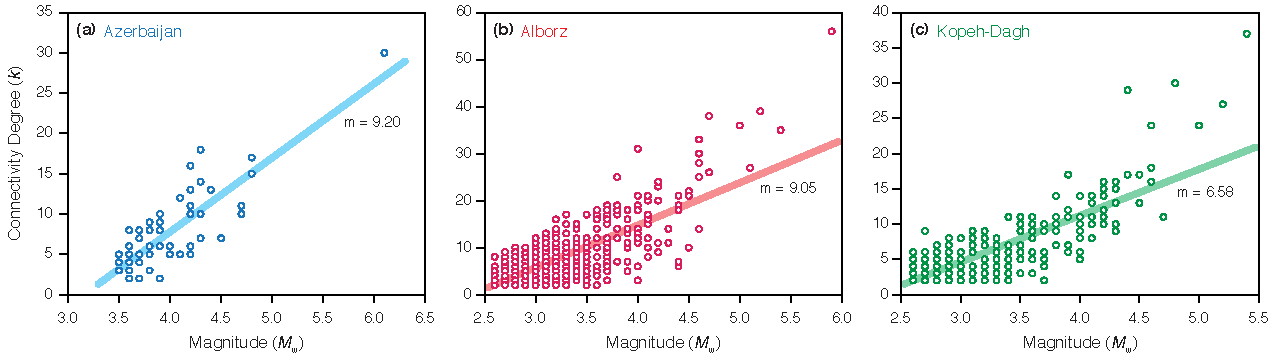
\includegraphics[width=\textwidth]{figures/pdf/figure-06} 
	\caption{$k-M$ relationship for north Iran tectonic seismic regions. The blue circles indicate the connectivity degrees. The red line is the linear regression line fits the data. The numbers on the lines is the slope of the regression lines.}
	\label{fig:km}
\end{figure*}

% We compared the  $k$-$M$  slope with the  $b$-value  of the Gutenberg-Richter law through the entire catalog and in the sliding windows in time. The $b$-value is generated through the maximum likelihood estimation \citep{Aki1965}.

% \begin{equation}
% 	b = \frac{log_{10}(e) }{\overline{M} - M_{min}},
% \end{equation}

% \noindent
% where $e$ is the mathematical constant, $\overline{M}$ is the average magnitude, and  $M_ {min}$ is the minimum magnitude in the sample, which in this case is the completeness magnitude for each tectonic seismic region. The number of sequences and threshold magnitudes is considerably different for all tectonic seismic regions.  \citet{Telesca2013}  studied the effect of the number of earthquakes in the catalog on the  $k-M$  slope. Comparing the result with the Guerrero region with reduced random sequence,  \citet{Telesca2013}  found that the number of sequences did not affect the  $k-M$  slope.  According to  \citet{Telesca2012}, the threshold magnitude has minor effect in the VG parameters.\\

% In order to analyze the sensitivity of the catalogs to the number of events and the threshold magnitude, we randomly picked 200 sequences from the catalogs with various sequence sizes. Number of events at each sequence should be low enough to be able to choose 200 random sequence from the catalog (note that the number of events in each catalog, before removing the events with magnitude less than the completeness magnitude, is 271, 1262, and 399 for Azerbaijan, Alborz, and Kopeh Dagh regions, respectively). Also it should be long enough to preserve the seismic characteristic of each tectonic seismic region. Based on mentioned criteria, we choose the minimum size of random windows as 150 events. The maximum size is the size of the entire catalog. The random sequences are consecutive, in other words, we randomly determine the initial event and sequence size, then we pick that size of event starting from the initial event. For each randomly picked magnitude time series,  we estimate $Mc$; then the $k-M$  and $b-value$ are calculated. Fig.~\ref{fig:random} shows the relationship between  $k-M$  slope and  $b-value$  of the randomly selected data and the statistical parameters for variables. Although changing the number of events and the threshold magnitude is slightly changing the results, however,  the results are fairly well clustered for each tectonic seismic region. 
   
\begin{figure*}%[t]
	\centering
	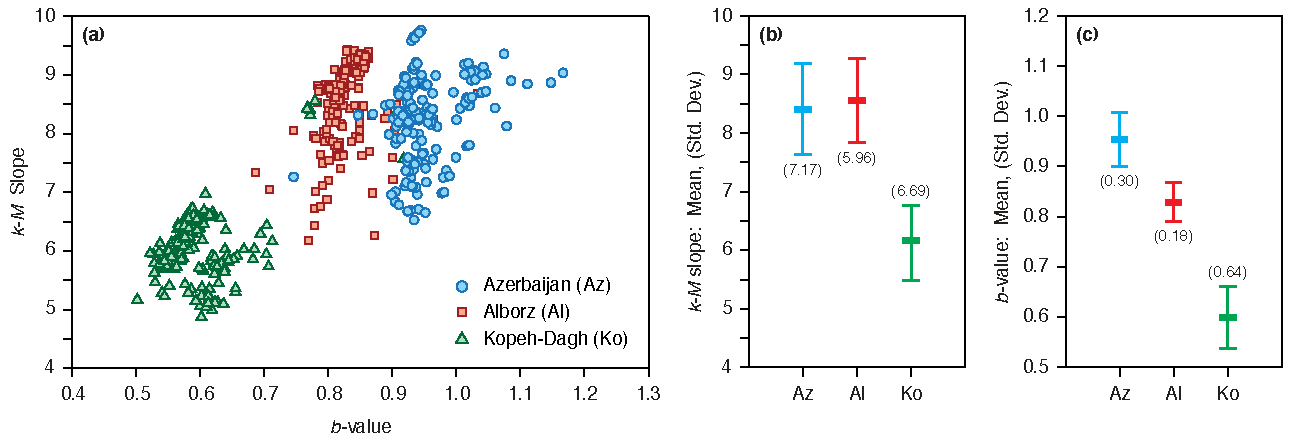
\includegraphics[width=0.9\textwidth]{figures/pdf/figure-07} 
	\caption{Relationship between $k-M$ and $b-value$ of three Iranian tectonic seismic regions for 200 random sequence. The numbers on the mean and standard deviation plots are coefficient of variations in percent $(standard \ deviation / mean)$.}
	\label{fig:random}
\end{figure*}

% The coefficient of variation of parameters is shown in Fig.~\ref{fig:random}. The  $k-M$  slope shows the higher coefficient of variation which indicates the fact that the  $k-M$  slope is more dependent on the window size and threshold magnitude than on the a-  and  b-values , which suggests that  the $k-M$  slope can better represent the dynamic characteristics of the magnitude-time series. 

% Fig.~\ref{fig:regression} shows the relationship between the  $k-M$  slope and $b-value$ for the three tectonic seismic regions in northern Iran and three other studies of Mexican zones  \citep{Telesca2013}, Pannonia zones  \citep{Telesca2014}, and synthetic data \citep{Telesca2014-pone}. Adding the results of the current study into the results of three previous similar studies improves the regression factor, and empowers the concept of the universal character of the relationship between the  $b-value$  and the  $k-M$  slope, as  \citet{Telesca2014} concluded. 
 
\begin{figure}[h]%[t]
	\centering
	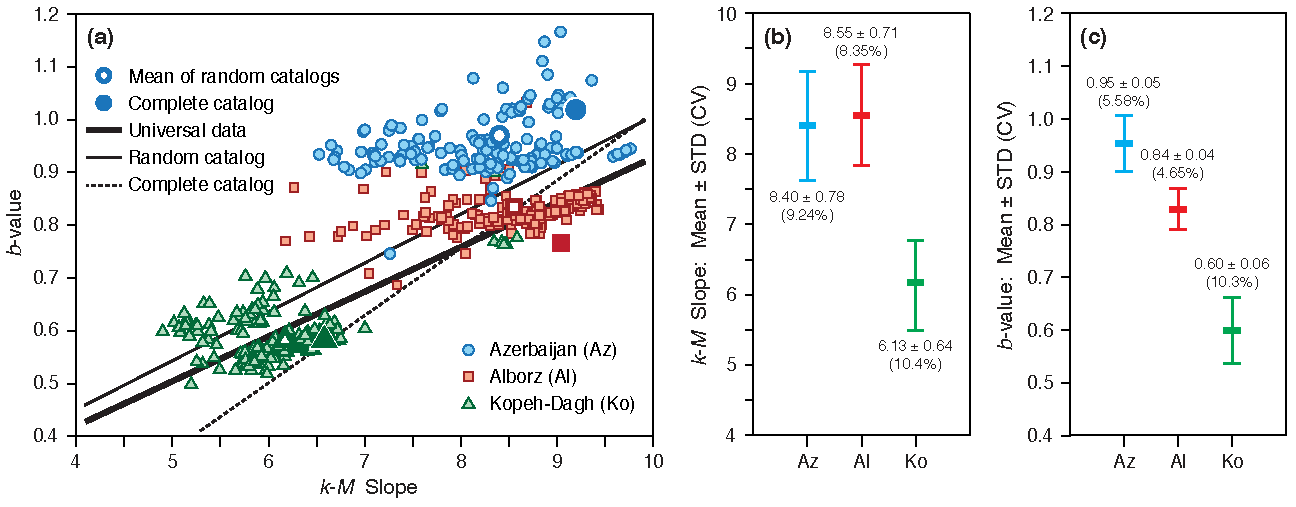
\includegraphics[width=0.45\textwidth]{figures/pdf/figure-08} 
	\caption{Relationship between $k-M$ slope and $b-value$ of three Iranian tectonic seismic zones (this study) and three other studies of Mexican zones \citep{Telesca2013}, Pannonia zones \citep{Telesca2014}, and synthetic data \citep{Telesca2014-pone}. The lines represent the linear regression fit of data. The correlation coefficients (R) are represented for different combination of data.}
	\label{fig:regression}
\end{figure}

% Fig.\ref{fig:tc} shows the variation of the  $k-M$  slope and  $b-value$  with time. Due to lower number of events in Azerbaijan's catalog, we choose 20 events as the window length with a shift of one event between two successive windows. With higher window length we loose the variation of considerable amount of information in time (e.g. with n=40 we loose almost half of the Azerbaijan catalog). Due to taking average values of successive windows, very small window length can not display the seismicity behavior especially before big earthquake. Maintaining consistency, we use the window length equal to 20 events for all three regions. The calculated parameters of each window are associated with the time of occurrence of the last event in the sliding window. The  $k-M$  slope and  $b-value$  in all tectonic seismic regions are very similar. In general, in all regions the $b-value$  and  $k-M$  slope drop considerably before large earthquakes. The decline in the  $b-value$  before large earthquakes has been studied in many regions \citep{Wyss2000, Wyss2006, Schorlemmer2005, Chan2012}.

% \citet{Telesca2016}  observed the decrease in  $<T_c>$  before the large earthquake of the western India earthquake sequence. Fig.\ref{fig:tc}  shows the time variation of  $<T_c>$   in the study area. The reduction of  $<T_c>$   before large earthquakes is clearly visible.  \citet{Telesca2016}  demonstrated that the decrement of  $<T_c>$   before a large earthquake is independent of window size and threshold magnitude. Decreasing the value of  $<T_c>$  ,  $k-M$ , and  $b-value$  before large earthquakes predominantly happened in all tectonic seismic regions (see Fig.\ref{fig:tc} for reference.)
 
% \begin{figure*}[t]
% 	\centering
% 	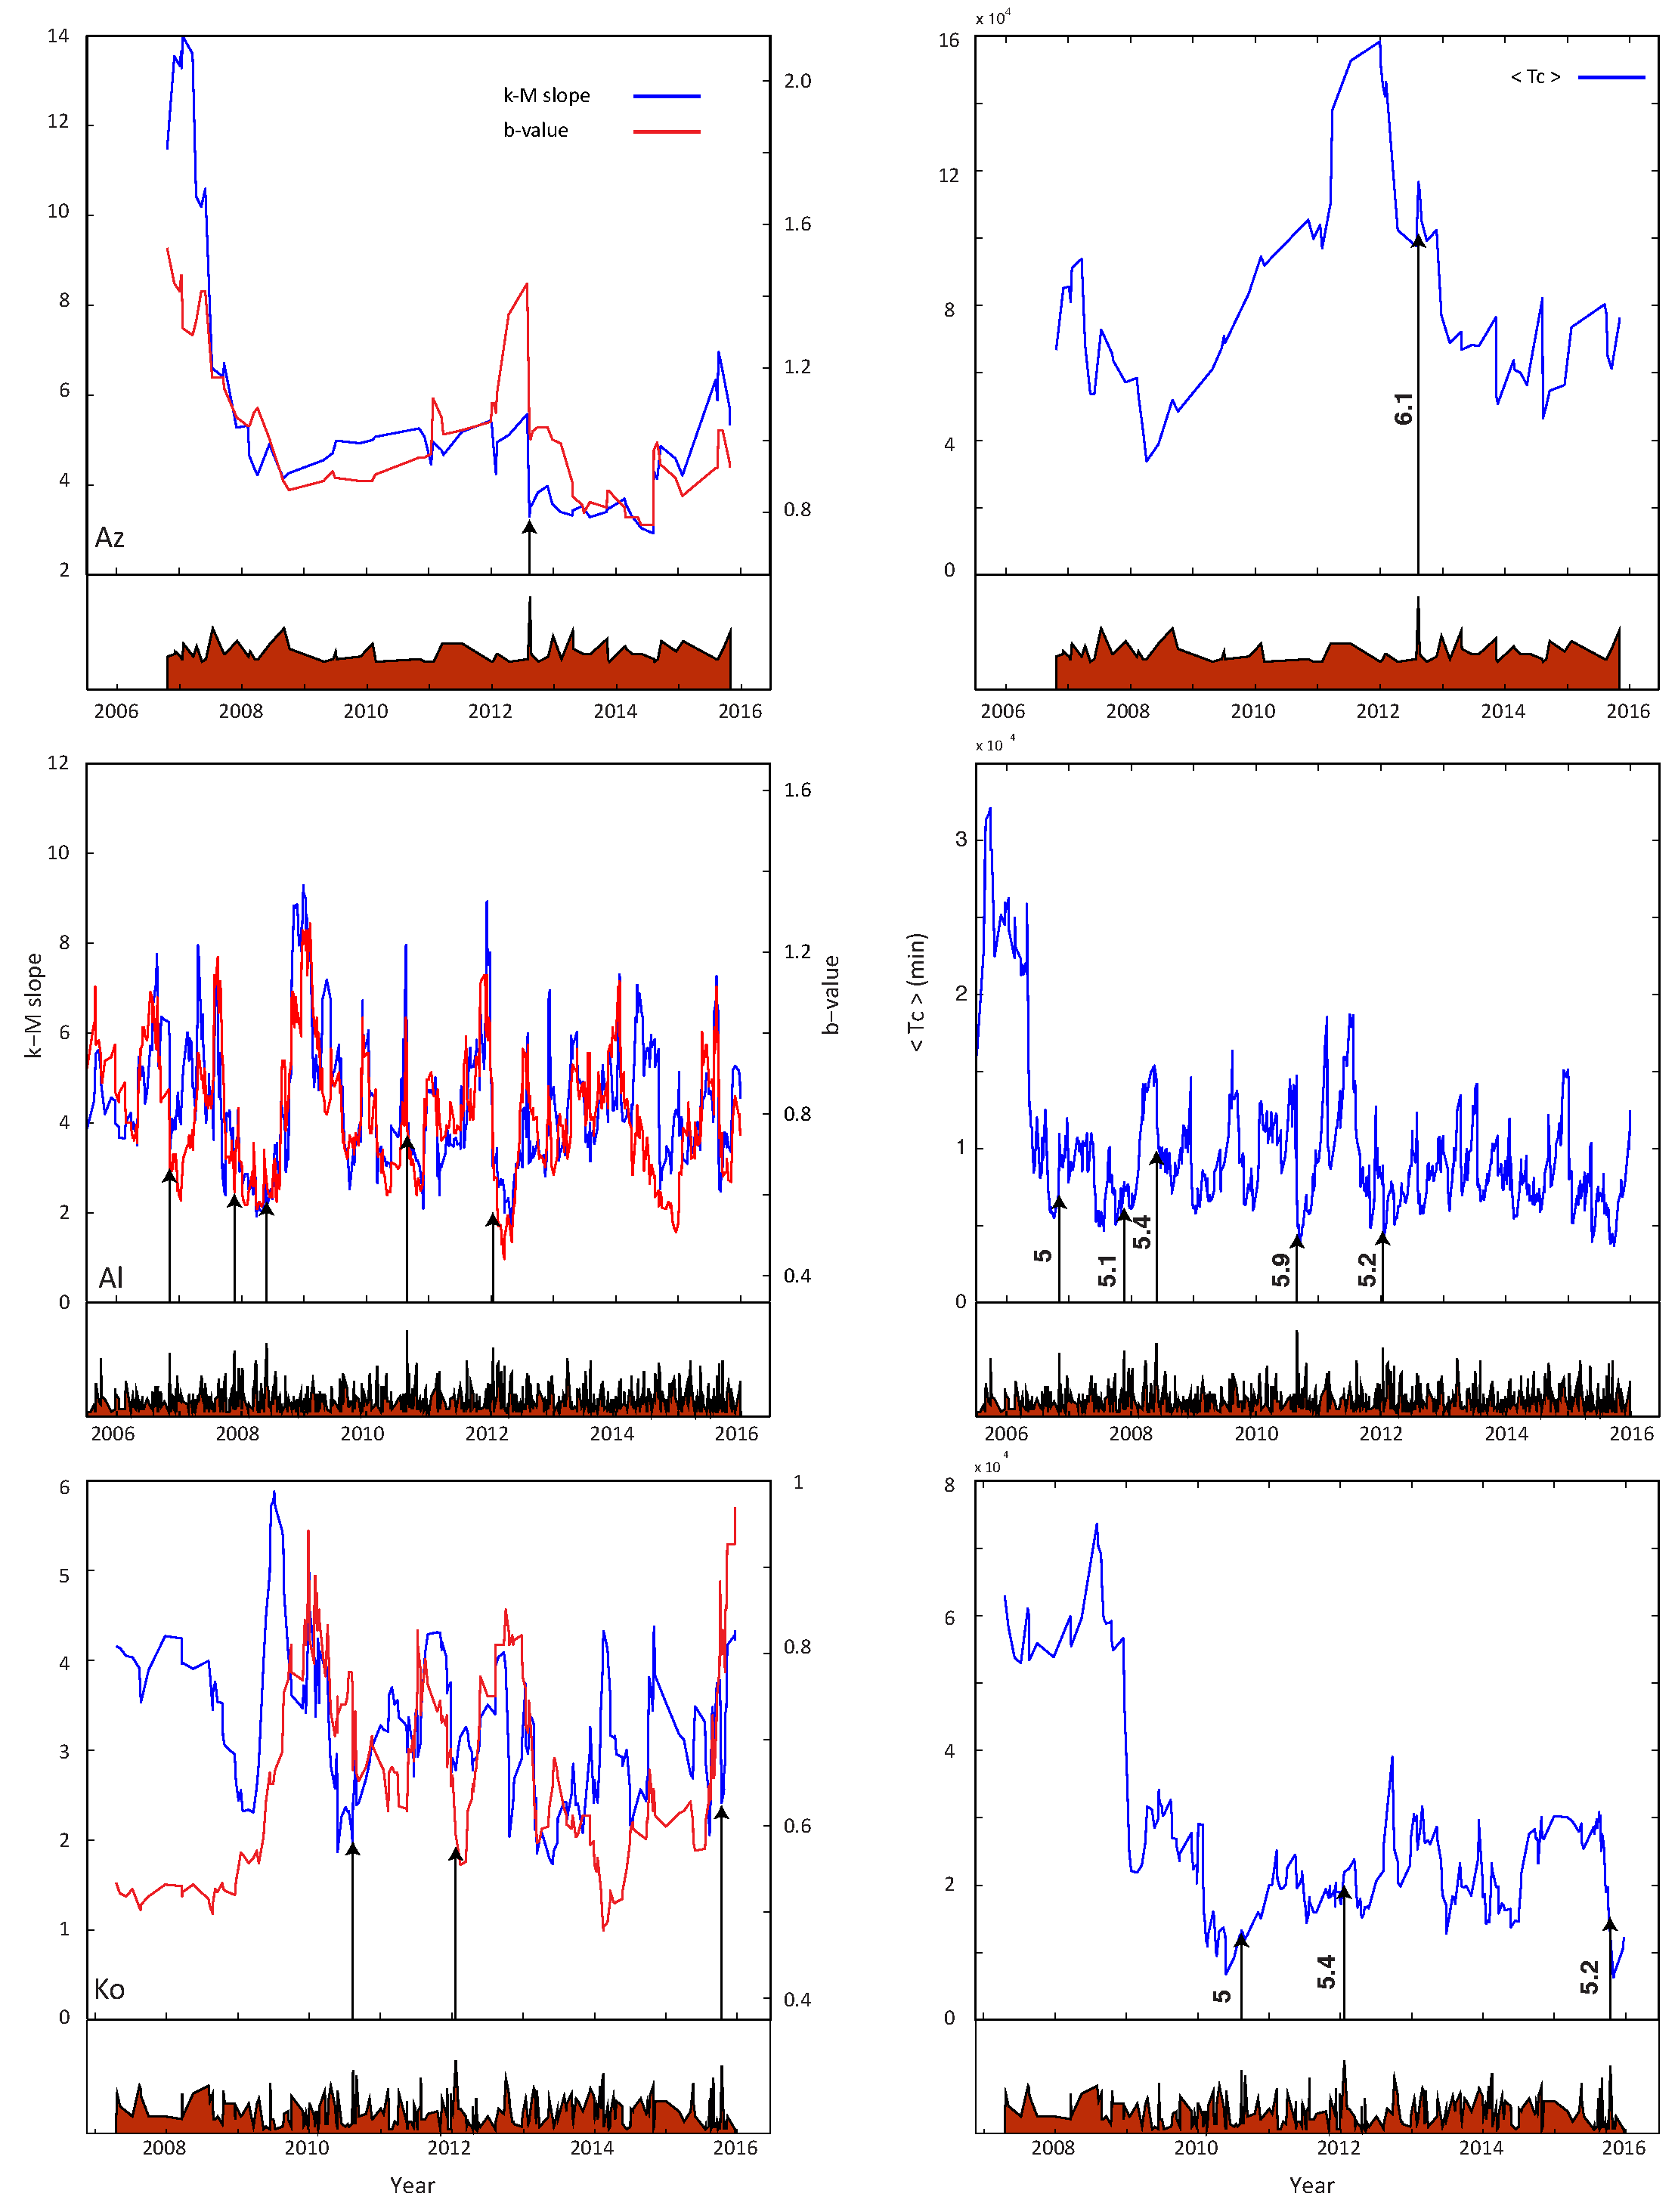
\includegraphics[scale=0.4]{figures/pdf/Figure10.pdf} 
% 	\caption{ Variation of $k-M$ slope  and $b-value$ (Left), and $ < T_c >$ (Right) as a function of time for three tectonic seismic regions in north Iran. Black arrows show the occurrence of the major earthquakes. Numbers on arrows indicate the moment magnitude of the earthquake (see Fig.~\ref{fig:mag-time} for reference).  The magnitude-time series are presented as a filled plot blew each plot. The variation of the heigh of filled plots are corresponding to the event magnitudes. Decreasing the value of  $<T_c>$  ,  $k-M$ , and  $b-value$  before large earthquakes predominantly happened in all tectonic seismic regions.}
% 	\label{fig:tc}
% \end{figure*}
